\section{Software Installation \& Ecosystem}
\subsection{Important Websites}

\frame
{
\frametitle{\url{http://libmesh.github.io}}

\centerline{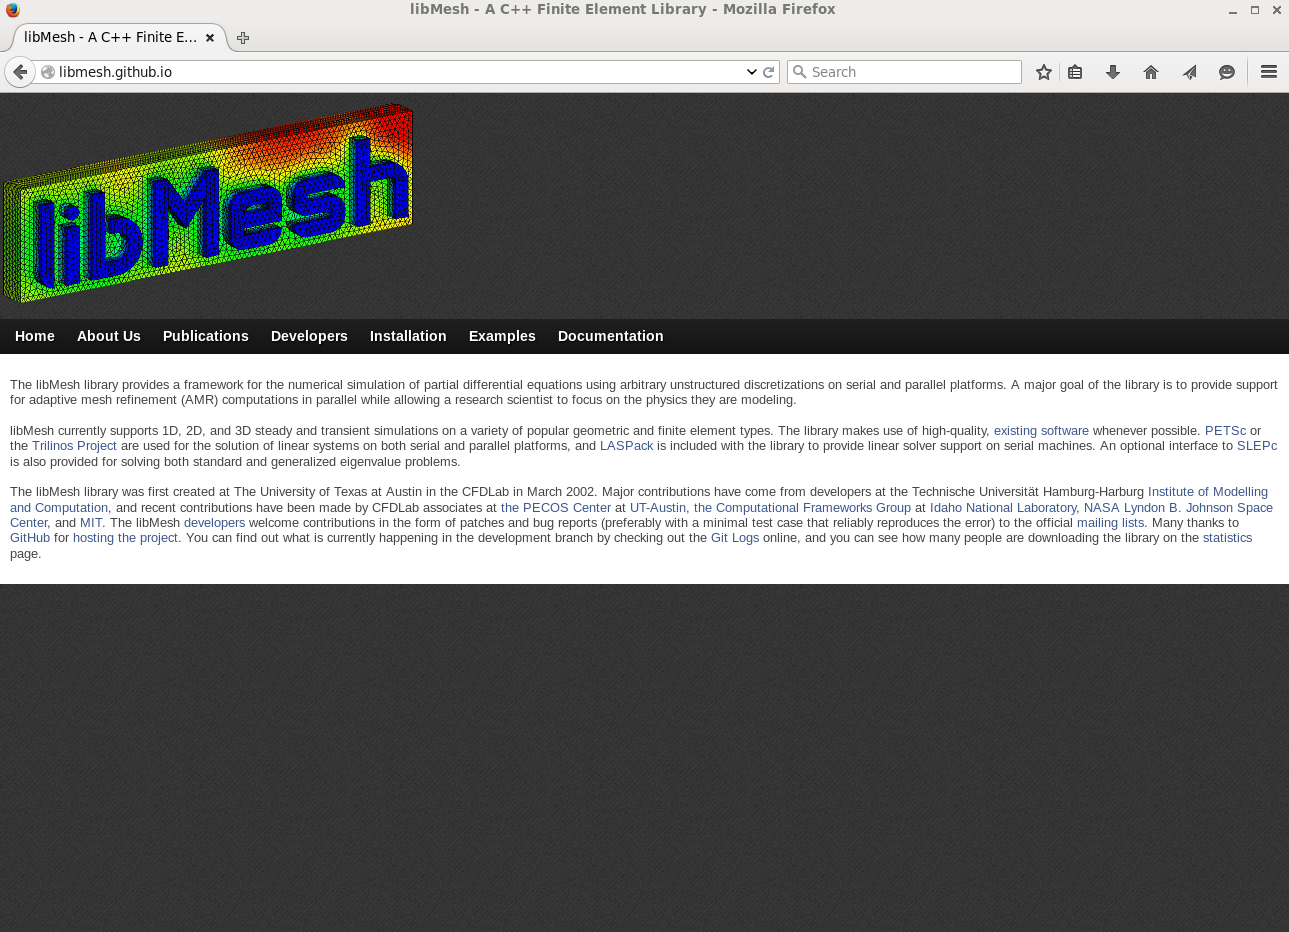
\includegraphics[width=0.85\textwidth]{webpage}}
}


\frame
{
\frametitle{\url{http://github.com/libMesh/libmesh}}

\centerline{\includegraphics[width=0.85\textwidth]{trivia/github_site}}
}


\frame
{
\frametitle{MooseBuild Testing Integrated with GitHub}

\centerline{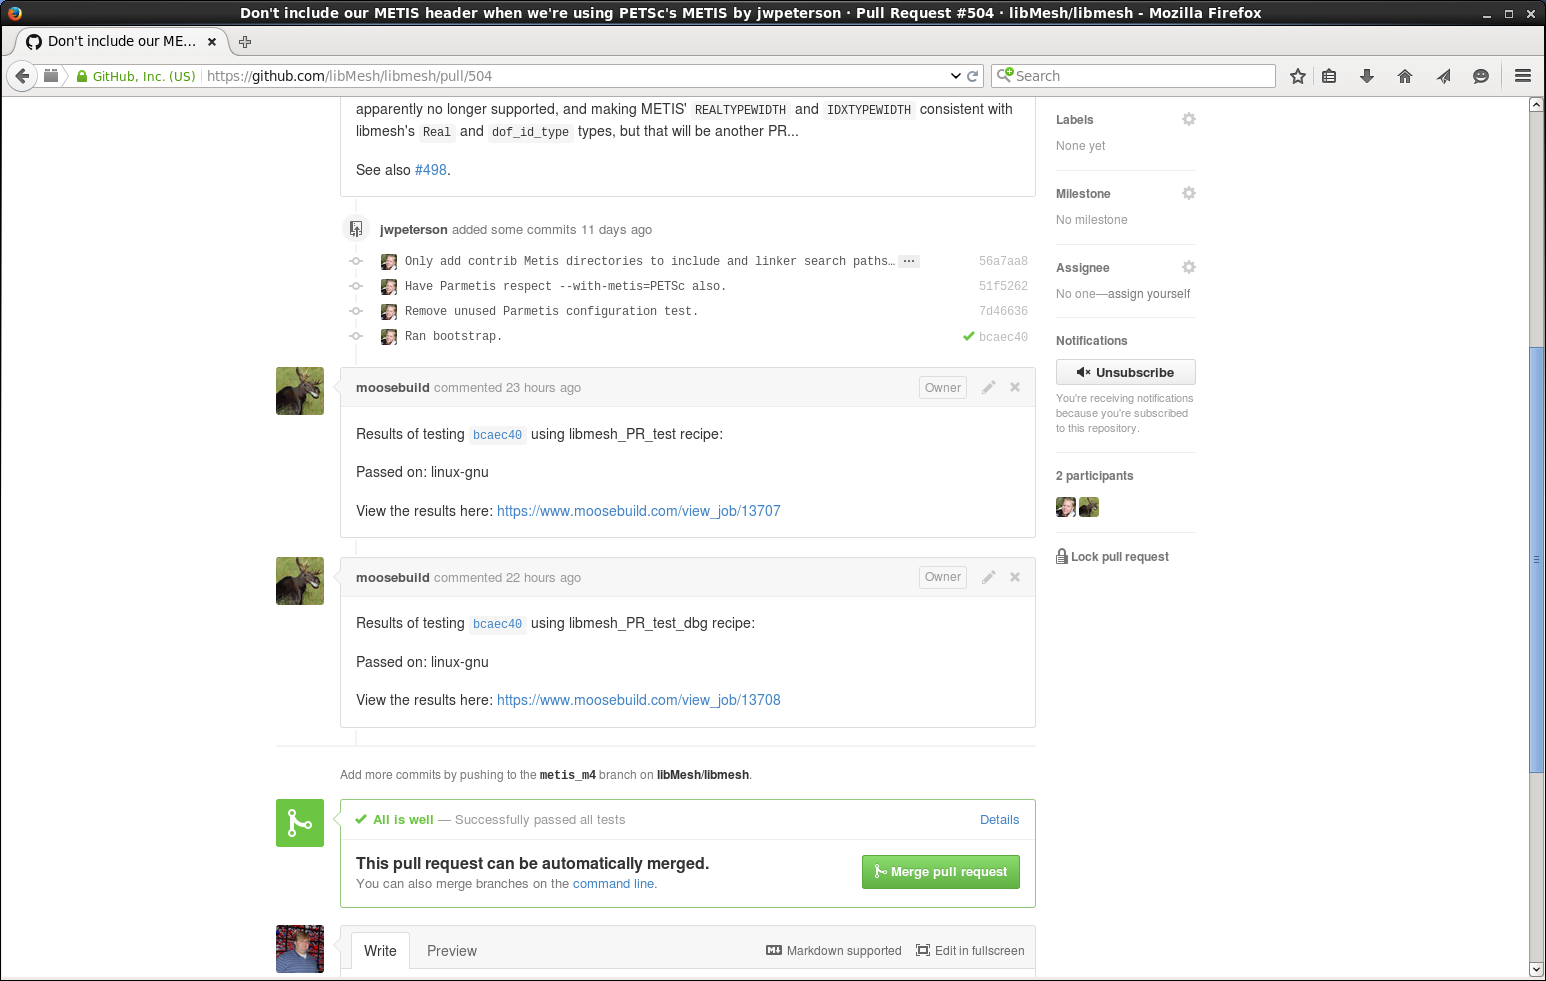
\includegraphics[width=0.85\textwidth]{moose_build}}
}



\subsection{Building the library}

\begin{frame}[fragile]
  \frametitle{Getting the \libMesh{} Source}

  \begin{block}{}
    \begin{itemize}
    \item \textbf{Blessed, Stable releases:}

      Download prepackaged releases from

      \scriptsize{\url{http://github.com/libMesh/libmesh/releases}}
      \normalsize
    \item \textbf{Development tree:}

      Grab the latest source tree from GitHub:
      \begin{lstlisting}[language=bash]
$ git clone git://github.com/libMesh/libmesh.git
      \end{lstlisting}
    \end{itemize}
  \end{block}
\end{frame}

\begin{frame}
  \frametitle{\libMesh{} Suggested Dependencies}
  \begin{itemize}
    \item  \texttt{MPI} is of course required for distributed-memory parallelism.
    \item Out of the box, \libMesh{} will build with support for serial linear systems.
    \item Highly recommended you first install \texttt{PETSc} and/or \texttt{Trilinos}, which \libMesh{} uses for solving linear systems in parallel.
      \item Other recommended, optional packages are:
        \begin{itemize}
          \item \texttt{SLEPc}: eigenvalue support on top of \texttt{PETSc}.
          \item Intel's Threading Building Blocks for shared-memory multithreading.
        \end{itemize}
  \end{itemize}
\end{frame}

\begin{frame}[fragile]
  \frametitle{Building \libMesh{} from source}

  \begin{block}{Unpack, Configure, Build, Install, \& Test}
    \begin{lstlisting}[language=bash]
# unpack the distribution
$ tar jxf libmesh-0.9.5.tar.bz2 && cd libmesh-0.9.5
# configure, install into the current directory
$ ./configure --prefix=$PWD/install
# build & install
$ make -j 4 && make -j 4 install
# run all the examples, but only the optimized flavor
$ make -j 4 check METHODS=opt
    \end{lstlisting}
  \end{block}
\end{frame}



